% \input{preambulo}
\documentclass[11pt]{article}
% Fonte em portgues brasileiro
\usepackage[brazilian]{babel}
\usepackage[utf8]{inputenc}
\usepackage[T1]{fontenc}
\usepackage{helvet} % Fonte usada neste template
\usepackage{ifthen}

% Pacote titlesec para formatação de titulos com a fonte utilizada
\usepackage{titlesec}
\titleformat{\chapter}[display]
  {\normalfont\sffamily\Large\bfseries\color{black}}
  {\chaptertitlename\ \thechapter}{20pt}{\Huge}
\titleformat{\section}
  {\normalfont\sffamily\large\bfseries\color{black}}
  {\thesection}{1em}{\Large}
\titleformat{\subsection}
  {\normalfont\sffamily\bfseries\color{black}}
  {\thesubsection}{1em}{\large}
\titleformat{\subsubsection}
  {\normalfont\sffamily\small\bfseries\color{black}}
  {\thesubsubsection}{1em}{}
% Tabelas
\usepackage{booktabs}
\usepackage{multirow}
\usepackage{multicol}
\usepackage{longtable}
\usepackage{makecell}
\usepackage{tabularx}
\usepackage[table]{xcolor}
\definecolor{color}{RGB}{156,28,36} % Cor padrão da Ageon


\newcolumntype{C}[1]{>{\centering\arraybackslash}p{\dimexpr#1-2\tabcolsep-2\arrayrulewidth}} % Tipo alternativo de coluna centralizada
\newcolumntype{P}[1]{>{\raggedright\arraybackslash}p{\dimexpr#1-2\tabcolsep-2\arrayrulewidth}} % Tipo alternativo de coluna justificada a direita


% Para inserir legenda de figuras dentro de tabelas
\makeatletter
\def\figcaption{%
\refstepcounter{figure}%
\@dblarg{\@caption{figure}}}
\makeatother

% Para inserir legenda de tabelas dentro de tabelas
\makeatletter
\def\tablecaption{%
\refstepcounter{table}%
\@dblarg{\@caption{table}}}
\makeatother

% Identação e espaçamento
\usepackage{pifont}
\usepackage{amssymb}
\usepackage[a4paper, headheight=50pt]{geometry}
\usepackage[headings]{fullpage}
\usepackage{indentfirst}   % Identar parágrafo em cada quebra de linha

% Figuras
\usepackage{graphicx}      % Pictures
\usepackage[font={footnotesize, sf}, labelfont={footnotesize, sf}]{caption}
\usepackage{transparent}

% Packages adicionais
\usepackage{listingsutf8}
\usepackage{inconsolata}
\usepackage{xcolor}
\usepackage{amsmath}
\usepackage{mathrsfs}
\usepackage{hyperref}
\usepackage[official]{eurosym}

% Estilo de página e rodapés
\usepackage{lastpage}
\usepackage{fancyhdr}
\pagestyle{fancy}
\fancyhf{}
\rhead{{\fontfamily{phv}\selectfont \footnotesize \transparent{0.6}\textbf{\textit{Vibration report}}}}
\lhead{\transparent{0.6}
\includegraphics[trim=1 1 1 1, clip, width=.15\linewidth]{figuras/logo.pdf}}

\rfoot{\fontfamily{phv}\selectfont \tiny \transparent{0.6}Page \thepage}
\lfoot{\fontfamily{phv}\selectfont \tiny \transparent{0.6}NBT AG \\ Switch vibration report}
\renewcommand{\footrulewidth}{0.4pt}

\usepackage{mdframed}
\renewcommand{\arraystretch}{1.2}

% Para utilização de itens enumerados com letras a), b), ...
\usepackage[shortlabels]{enumitem}

\begin{document}
{\fontfamily{phv}\selectfont
\newpage
\lstset{ literate={â}{{\^{a}}}1 {Â}{{\^{A}}}1 {ç}{{\c{c}}}1 {Ç}{{\c{C}}}1 {ğ}{{\u{g}}}1 {Ğ}{{\u{G}}}1 {ı}{{\i}}1 {İ}{{\.{I}}}1 {ö}{{\"o}}1 {Ö}{{\"O}}1 {ş}{{\c{s}}}1 {Ş}{{\c{S}}}1 {ü}{{\"u}}1 {Ü}{{\"U}}1 }

\begingroup
\centering
\setlength{\tabcolsep}{1pt} % Default value: 6pt
\setlength\arrayrulewidth{1pt}
\renewcommand{\arraystretch}{1.5} % Default value: 1
\begin{tabularx}{\textwidth}{|C{\textwidth}|}
\hline
\rowcolor{color}
\textbf{\color{white}\Large Switch Vibration Report}\\
\hline
\end{tabularx}

\vspace{\belowdisplayskip}
 \begin{footnotesize}
\begin{tabularx}\textwidth{ |p{0.4\textwidth}|X| }
\hline
\textbf{Switch ID} & switch_id \\ \hline
\textbf{Device ID} & dev_id \\ \hline
\textbf{Date} & date \\ \hline
    \textbf{Total number of events} & _events \\ \hline
\end{tabularx}
 \end{footnotesize}
\endgroup

\section{Maximum RMS values registered on the day}
\begin{center}
%\begin{Large}
    \begin{tabularx}\textwidth{ |p{0.4\textwidth}|X| }
\hline
\textbf{Axis} & \textbf{Values ($m/s^2$)} \\ \hline
Transversal (X-axis) & rms_x_avg \\ \hline
Longitudinal (Y-axis) & rms_y_avg \\ \hline
Vertical (Z-axis) & rms_z_avg \\ \hline
\end{tabularx}
%\end{Large}
\end{center}



%\section{Maximum RMS Values}
%\begin{center}
%\begin{Large}
%    \begin{tabularx}\textwidth{ |p{0.4\textwidth}|X| }
%\hline
%\textbf{Axis} & \textbf{Values ($m/s^2$)} \\ \hline
%Transversal (X-axis) & rms_x_max \\ \hline
%Longitudinal (Y-axis) & rms_y_max \\ \hline
%Vertical (Z-axis) & rms_z_max \\ \hline
%\end{tabularx}
%\end{Large}
%\end{center}
%\newpage
\section{Raw data of all events}
Raw data of all events occurred. The horizontal axis does not represent time, but all the events bundled together.
To get a glimpse of how many events happened during the day and the RMS values for each event, refer to the next section.

\begin{figure}[!ht]
\centering
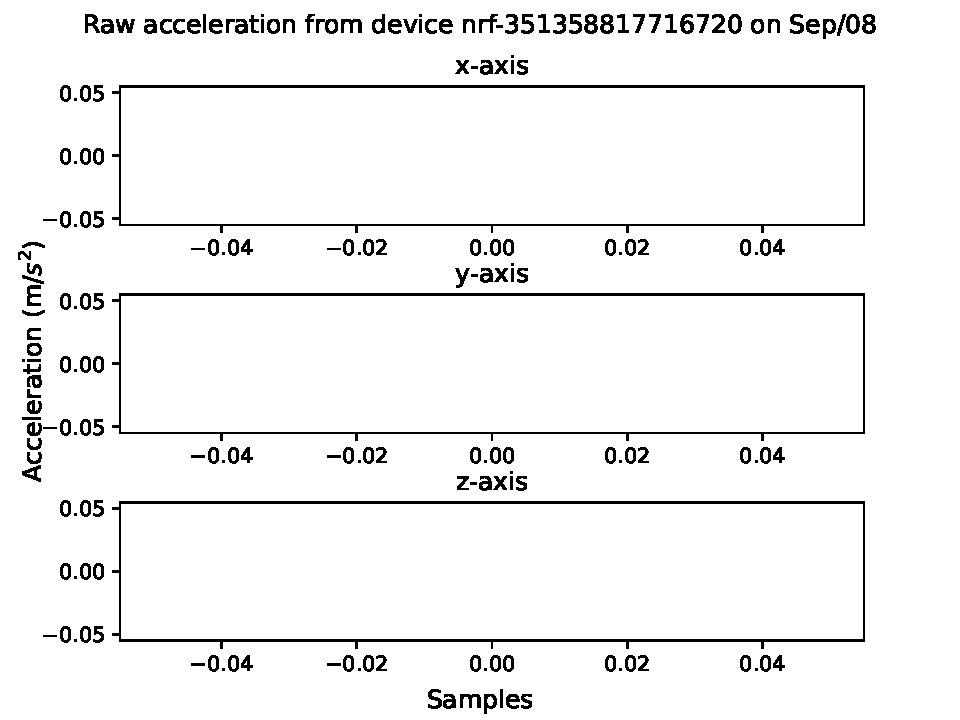
\includegraphics[width=.9\linewidth]{figuras/Figure_1.pdf}
% \fontfamily{phv}\selectfont\caption{Determinação dos limites de operação do produto.}
\label{fig:lim1}
\end{figure}
\newpage
\section{RMS values for each individual event}
Each bar in the graph indicates an individual event

\begin{figure}[!ht]
\centering
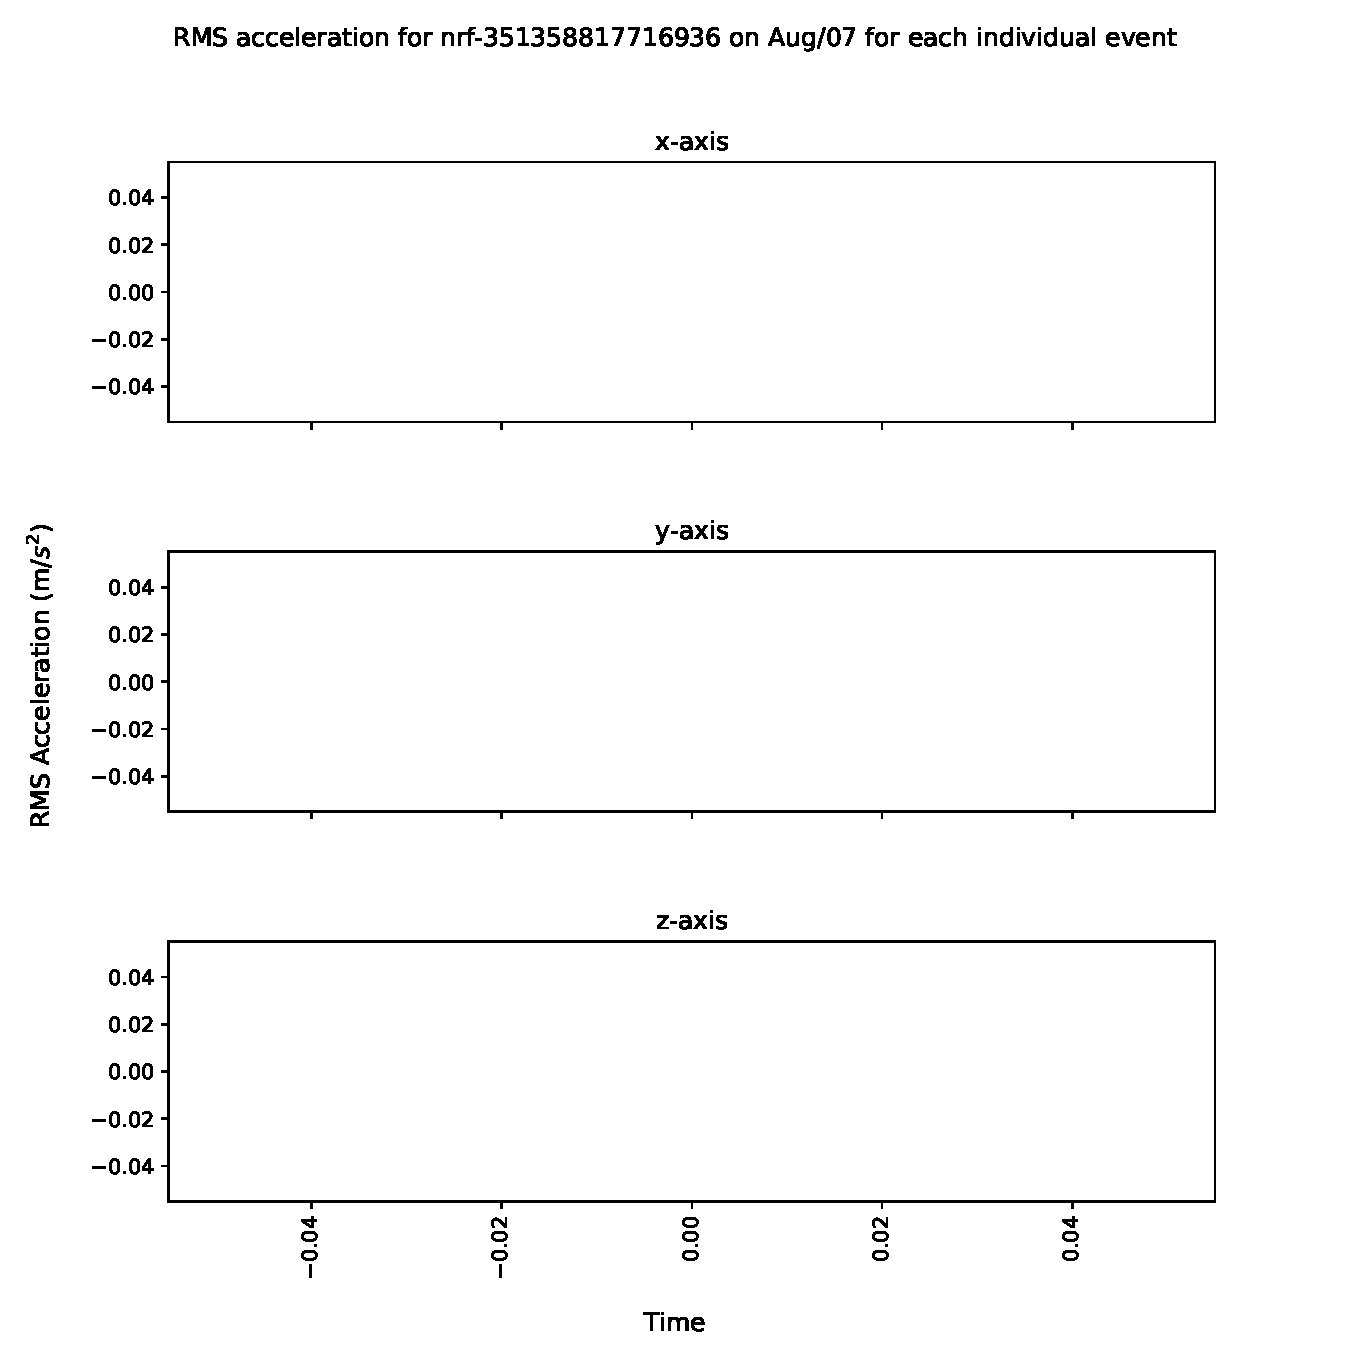
\includegraphics[width=.9\linewidth]{figuras/Figure_2.pdf}
% \fontfamily{phv}\selectfont\caption{Determinação dos limites de operação do produto.}
\label{fig:lim}
\end{figure}


\end{document}